\section{Visão elementar sobre estabilidade transitória}
\begin{frame}
\frametitle{Sistema de barramento infinito para uma máquina}
\begin{figure}[h!]
\begin{center}
    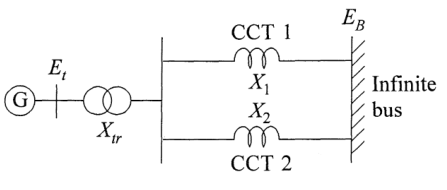
\includegraphics[width=10cm]{imagens/maq1.png}  
\end{center}
%\caption{Resultado prático da planta em malha aberta.}
\label{maq1} 
\end{figure}
\end{frame}
	
\begin{frame}

\begin{figure}[h!]
\begin{left}
    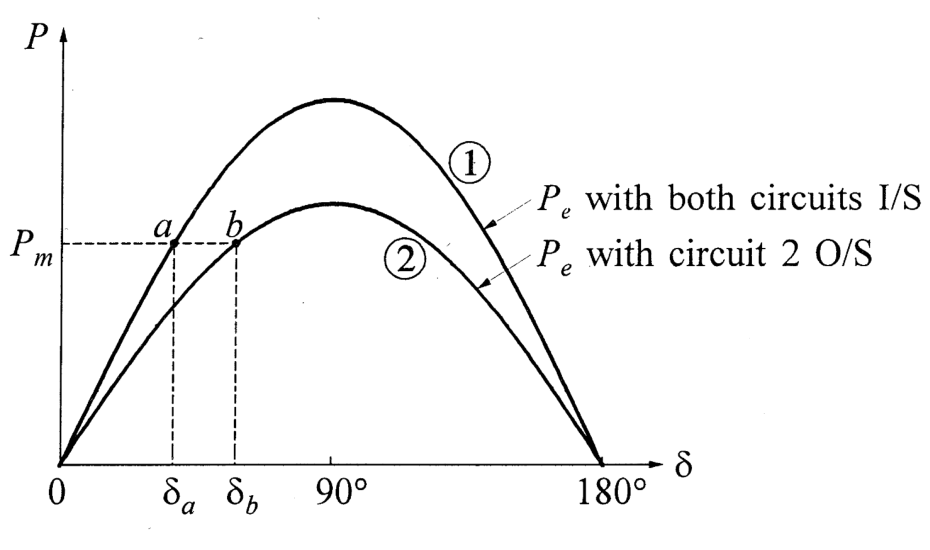
\includegraphics[width=10cm]{imagens/maq4.png}  
\end{left}
%\caption{Resultado prático da planta em malha aberta.}
\label{maq4} 
\end{figure}


\frametitle{Relação entre o ângulo de potência}
\begin{textblock*}{10pt}(300pt,40pt)
\small
\begin{equation*}
   P_{e}=\frac{E^{'}E_B}{X_T}sen(\delta)
\end{equation*}
\end{textblock*}
\end{frame}



\begin{comment}
\begin{frame}
\frametitle{Circuito equivalente}
\begin{figure}[h!]
\begin{center}
    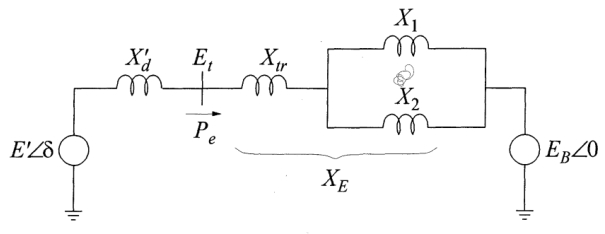
\includegraphics[width=10cm]{imagens/maq2.png}  
\end{center}
%\caption{Resultado prático da planta em malha aberta.}
\label{maq2} 
\end{figure}
\end{frame}
	
\begin{frame}
\frametitle{Circuito equivalente reduzido}
\begin{figure}[h!]
\begin{center}
    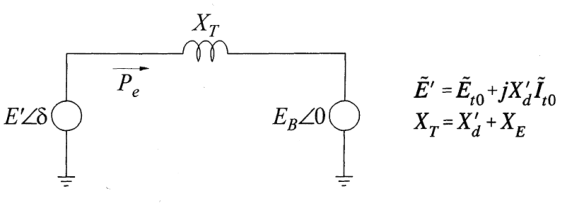
\includegraphics[width=10cm]{imagens/maq3.png}  
\end{center}
%\caption{Resultado prático da planta em malha aberta.}
\label{maq3} 
\end{figure}
\end{frame}


\end{comment}	
